% !TeX document-id = {c68f4be8-c497-43e0-82df-e9ebfbea9577}
% !TeX TXS-program:pdflatex = pdflatex -synctex=1 -interaction=nonstopmode --shell-escape %.tex
% новая команда \RNumb для вывода римских цифр
\documentclass[a4paper,12pt]{article}
\usepackage{amssymb}
\usepackage{amsmath}
\usepackage{amsthm}
\usepackage{caption}
\usepackage{misccorr}
\usepackage[noadjust]{cite}
\usepackage{cmap}
\usepackage[utf8x]{inputenc}
\usepackage[T2A]{fontenc}
\usepackage[english, russian]{babel}
\usepackage{graphics}
\usepackage{graphicx}
\usepackage{textcomp}
\usepackage{verbatim}
\usepackage{makeidx}
\usepackage{geometry}
\usepackage{float}
\usepackage{bm}
\usepackage{esint}
\usepackage{mathtools}
\usepackage{graphicx}
\usepackage{listings}
\usepackage{courier}
\usepackage{multirow}
\usepackage{graphicx}
\usepackage{xcolor}
\usepackage{ucs}


\lstdefinestyle{asm}{
	language={[x86masm]Assembler},
	backgroundcolor=\color{white},
	basicstyle=\footnotesize\ttfamily,
	keywordstyle=\color{blue},
	stringstyle=\color{red},
	commentstyle=\color{gray},
	numbers=left,
	numberstyle=\tiny,
	stepnumber=1,
	numbersep=5pt,
	frame=single,
	tabsize=4,
	captionpos=b,
	breaklines=true
}

\lstset{basicstyle=\fontsize{10}{10}\selectfont,breaklines=true,inputencoding=utf8x,extendedchars=\true}

\lstset{
	literate=
	{а}{{\selectfont\char224}}1
	{б}{{\selectfont\char225}}1
	{в}{{\selectfont\char226}}1
	{г}{{\selectfont\char227}}1
	{д}{{\selectfont\char228}}1
	{е}{{\selectfont\char229}}1
	{ё}{{\"e}}1
	{ж}{{\selectfont\char230}}1
	{з}{{\selectfont\char231}}1
	{и}{{\selectfont\char232}}1
	{й}{{\selectfont\char233}}1
	{к}{{\selectfont\char234}}1
	{л}{{\selectfont\char235}}1
	{м}{{\selectfont\char236}}1
	{н}{{\selectfont\char237}}1
	{о}{{\selectfont\char238}}1
	{п}{{\selectfont\char239}}1
	{р}{{\selectfont\char240}}1
	{с}{{\selectfont\char241}}1
	{т}{{\selectfont\char242}}1
	{у}{{\selectfont\char243}}1
	{ф}{{\selectfont\char244}}1
	{х}{{\selectfont\char245}}1
	{ц}{{\selectfont\char246}}1
	{ч}{{\selectfont\char247}}1
	{ш}{{\selectfont\char248}}1
	{щ}{{\selectfont\char249}}1
	{ъ}{{\selectfont\char250}}1
	{ы}{{\selectfont\char251}}1
	{ь}{{\selectfont\char252}}1
	{э}{{\selectfont\char253}}1
	{ю}{{\selectfont\char254}}1
	{я}{{\selectfont\char255}}1
	{А}{{\selectfont\char192}}1
	{Б}{{\selectfont\char193}}1
	{В}{{\selectfont\char194}}1
	{Г}{{\selectfont\char195}}1
	{Д}{{\selectfont\char196}}1
	{Е}{{\selectfont\char197}}1
	{Ё}{{\"E}}1
	{Ж}{{\selectfont\char198}}1
	{З}{{\selectfont\char199}}1
	{И}{{\selectfont\char200}}1
	{Й}{{\selectfont\char201}}1
	{К}{{\selectfont\char202}}1
	{Л}{{\selectfont\char203}}1
	{М}{{\selectfont\char204}}1
	{Н}{{\selectfont\char205}}1
	{О}{{\selectfont\char206}}1
	{П}{{\selectfont\char207}}1
	{Р}{{\selectfont\char208}}1
	{С}{{\selectfont\char209}}1
	{Т}{{\selectfont\char210}}1
	{У}{{\selectfont\char211}}1
	{Ф}{{\selectfont\char212}}1
	{Х}{{\selectfont\char213}}1
	{Ц}{{\selectfont\char214}}1
	{Ч}{{\selectfont\char215}}1
	{Ш}{{\selectfont\char216}}1
	{Щ}{{\selectfont\char217}}1
	{Ъ}{{\selectfont\char218}}1
	{Ы}{{\selectfont\char219}}1
	{Ь}{{\selectfont\char220}}1
	{Э}{{\selectfont\char221}}1
	{Ю}{{\selectfont\char222}}1
	{Я}{{\selectfont\char223}}1
}

\newcommand{\specchapter}[1]{\chapter*{#1}\addcontentsline{toc}{chapter}{#1}}
\newcommand{\specsection}[1]{\section*{#1}\addcontentsline{toc}{section}{#1}}
\newcommand{\specsubsection}[1]{\subsection*{#1}\addcontentsline{toc}{subsection}{#1}}
\newcommand{\RNumb}[1]{\uppercase\expandafter{\romannumeral #1\relax}}
\newcommand{\jj}{\righthyphenmin=20 \justifying}


% геометрия
\geometry{pdftex, left = 2cm, right = 2cm, top = 2.5cm, bottom = 2.5cm}

\setcounter{tocdepth}{4} % фикс переноса 
\righthyphenmin = 2
\tolerance = 2048

\begin{document}
\thispagestyle{empty}

\noindent \begin{minipage}{0.15\textwidth}
	
\includegraphics[width=\linewidth]{b_logo}
\end{minipage}
\noindent\begin{minipage}{0.9\textwidth}\centering
	\textbf{Министерство науки и высшего образования Российской Федерации}\\
	\textbf{Федеральное государственное бюджетное образовательное учреждение высшего образования}\\
	\textbf{«Московский государственный технический университет имени Н.Э.~Баумана}\\
	\textbf{(национальный исследовательский университет)»}\\
	\textbf{(МГТУ им. Н.Э.~Баумана)}
\end{minipage}

\noindent\rule{18cm}{3pt}
\newline\newline
\noindent ФАКУЛЬТЕТ $\underline{\text{«Информатика и системы управления»}}$ \newline\newline
\noindent КАФЕДРА $\underline{\text{«Программное обеспечение ЭВМ и информационные технологии»}}$\newline\newline\newline\newline\newline\newline\newline


\begin{center}
	\noindent\begin{minipage}{1.3\textwidth}\centering
	\Large\textbf{   ~~~ Лабораторная работа №1}\newline
	\textbf{по дисциплине "Операционные системы"}\newline\newline\newline
	\end{minipage}
\end{center}

\noindent\textbf{Тема} $\underline{\text{Дизассемблирование INT 8h}}$\newline\newline
\noindent\textbf{Студент} $\underline{\text{Романов А.В.}}$\newline\newline
\noindent\textbf{Группа} $\underline{\text{ИУ7-53Б}}$\newline\newline
\noindent\textbf{Преподаватель} $\underline{\text{Рязанова Н.Ю.}}$\newline

\begin{center}
	\vfill
	Москва~---~\the\year
~г.
\end{center}
\clearpage

\section{Полученный дизассемблированный код}

\subsection{Листинг INT8h} 
\begin{lstlisting}[style={asm}]
	; -- Вызов sub_1
	020A:0746  E8 0070              call    sub_1; (07B9) 
	; -- Сохранение регистров es, ds, ax, dx
	020A:0749  06                   push    es
	020A:074A  1E                   push    ds
	020A:074B  50                   push    ax
	020A:074C  52                   push    dx
	; -- Загрузка в DS 0040H
	020A:074D  B8 0040              mov ax,40h
	020A:0750  8E D8                mov ds,ax
	; -- AX = ES = 0
	020A:0752  33 C0                xor ax,ax; Zero register
	020A:0754  8E C0                mov es,ax
	; -- Инкрементирование счётчика таймера, по адресу 0040:006C
	020A:0756  FF 06 006C           inc word ptr ds:[6Ch; (0040:006C=5AEBh)
	020A:075A  75 04                jnz loc_1; Jump if not zero
	; -- Инкрементирование старших 2 байта счётчика таймера
	020A:075C  FF 06 006E           inc word ptr ds:[6Eh]; (0040:006E=2)
	; -- Проверка, что прошло 24 часа:
	;    0040H:006EH == 18H и 0040H:006CH == 00B0H
	;    24 * 60 * 60 * t == 18H << 16 + B0H, t - количество вызовов таймера в секунду
	020A:0760               loc_1:
	020A:0760  83 3E 006E 18        cmp word ptr ds:[6Eh],18h; (0040:006E=2)
	020A:0765  75 15                jne loc_2; Jump if not equal
	020A:0767  81 3E 006C 00B0      cmp word ptr ds:[6Ch],0B0h; (0040:006C=5AEBh)
	020A:076D  75 0D                jne loc_2; Jump if not equal
	; -- Зануление счётчика таймера, и занесение 1 в 0040H:0070H по прошествии 24 часов.
	020A:076F  A3 006E              mov word ptr ds:[6Eh],ax    ; (0040:006E=2)
	020A:0772  A3 006C              mov word ptr ds:[6Ch],ax    ; (0040:006C=5AEBh)
	020A:0775  C6 06 0070 01        mov byte ptr ds:[70h],1 ; (0040:0070=0)
	; -- AL = 8, т.к. до этой строчки AL = 0.
	020A:077A  0C 08                or  al,8
	020A:077C               loc_2:
	; -- Сохранение регистра AX
	020A:077C  50                   push    ax
	; -- Декрементирование счетчика отключения моторчика
	020A:077D  FE 0E 0040           dec byte ptr ds:[40h]; (0040:0040=0F7h)
	020A:0781  75 0B                jnz loc_3; Jump if not zero
	; -- Установка флагов, отвечающих за отключение моторчика дисковода
	020A:0783  80 26 003F F0        and byte ptr ds:[3Fh],0F0h; (0040:003F=0)
	; -- Отправить команду отключения моторчика дисковода
	020A:0788  B0 0C                mov al,0Ch
	020A:078A  BA 03F2              mov dx,3F2h
	020A:078D  EE                   out dx,al; port 3F2h, dsk0 contrl output
	020A:078E               loc_3:
	; -- Восстановление регистра AX
	020A:078E  58                   pop ax
	; -- Проверка 2 бита (Parity Flag)
	020A:078F  F7 06 0314 0004      test    word ptr ds:[314h],4; (0040:0314=3200h)
	020A:0795  75 0C                jnz loc_4; Jump if not zero
	; -- Загрузка младшего байта FLAGS в регистр AH
	020A:0797  9F                   lahf; Load ah from flags
	; -- Обмен ah и al. Таким образом: AX = 08[AH], [AH] - младший байт регистра FALGS
	020A:0798  86 E0                xchg    ah,al
	; -- Сохранение регистра AX
	020A:079A  50                   push    ax
	; -- Вызов 1CH с помощью адреса в таблице векторов. 
	;    При вызове через int произошел бы пуш регистра FLAGS в стек, 
	;    а в случае через call на его месте будет лежать положенный до AX,
	;    который по выходу из 1CH будет установлен в FLAGS с помощью iret.
	020A:079B  26: FF 1E 0070       call dword ptr es:[70h]
	020A:07A0  EB 03                jmp short loc_5; (07A5)
	020A:07A2  90                   nop
	020A:07A3               loc_4:
	020A:07A3  CD 1C                int 1Ch; Timer break (call each 18.2ms)
	020A:07A5               loc_5:
	020A:07A5  E8 0011              call    sub_1; (07B9)
	; -- Сброс контроллера прерываний.
	020A:07A8  B0 20                mov al,20h
	020A:07AA  E6 20                out 20h,al; port 20h, 8259-1 int command
	; -- Востановление регистров dx, ax, ds, es
	020A:07AC  5A                   pop dx
	020A:07AD  58                   pop ax
	020A:07AE  1F                   pop ds
	020A:07AF  07                   pop es
	020A:07B0  E9 FE99              jmp $-164h ; (020A:07B0h - 164h = 020A:064Ch)
	; ..........
	020A:064C  1E                   push    ds
	020A:064D  50                   push    ax
	; ...........
	020A:06AA  58                   pop ax
	020A:06AB  1F                   pop ds
	; -- Возврат из прерывания
	020A:06AC  CF                   iret; Interrupt return
\end{lstlisting}

\clearpage
\subsection{Листинг процедуры sub\_1}

\begin{lstlisting}[style={asm}]
	sub_1       proc    near
	; Сохранение регистров dx, ax
	020A:07B9  1E                   push    ds
	020A:07BA  50                   push    ax
	; -- AX = DS = 0040H
	020A:07BB  B8 0040              mov ax,40h
	020A:07BE  8E D8                mov ds,ax
	; -- Сохранение младшего байта FLAGS в AH
	020A:07C0  9F                   lahf; Load ah from flags
	; -- Проверка флага DF или старшего бита IOPL.
	;    Если кто-то установлен хотя бы один, то IF сбрасыватся через cli
	020A:07C1  F7 06 0314 2400      test    word ptr ds:[314h],2400h    ; (0040:0314=3200h)
	020A:07C7  75 0C                jnz loc_7; Jump if not zero
	; -- Сброс Interrput Enable Flag (9 бит - занулить). 
	;    lock для того чтобы команда была неделимой.
	020A:07C9  F0> 81 26 0314 FDFF  lock and word ptr ds:[314h],0FDFFh  ; (0040:0314=3200h)
	020A:07D0               loc_6:
	; -- Загрузка AH в  младший байт FLAGS.
	020A:07D0  9E                   sahf; Store ah into flags
	020A:07D1  58                   pop ax
	020A:07D2  1F                   pop ds
	020A:07D3  EB 03                jmp short loc_8; (07D8)
	020A:07D5               loc_7:
	; -- Сброс Interrput Enable Flag с помощью cli.
	020A:07D5  FA                   cli; Disable interrupts
	020A:07D6  EB F8                jmp short loc_6; (07D0)
	020A:07D8               loc_8:
	; -- Возврат из подпрограммы.
	020A:07D8  C3                   retn
	sub_1       endp
\end{lstlisting}
\clearpage

\section{Схема алгоритмов}

\subsection{Схема алгоритма обработчика INT8h}
""\newline

\begin{flushright}
	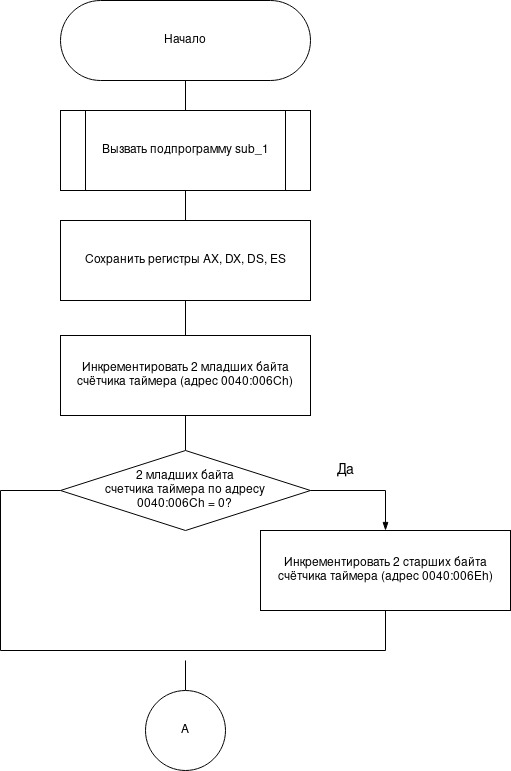
\includegraphics[scale=0.76]{../src/int8h_1.jpg}
	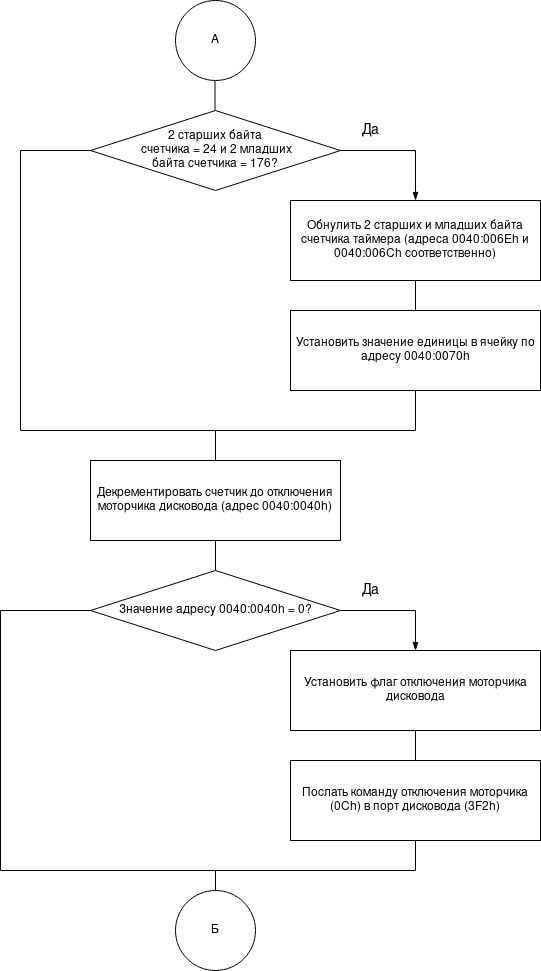
\includegraphics[scale=0.735]{../src/int8h_2.jpg}
	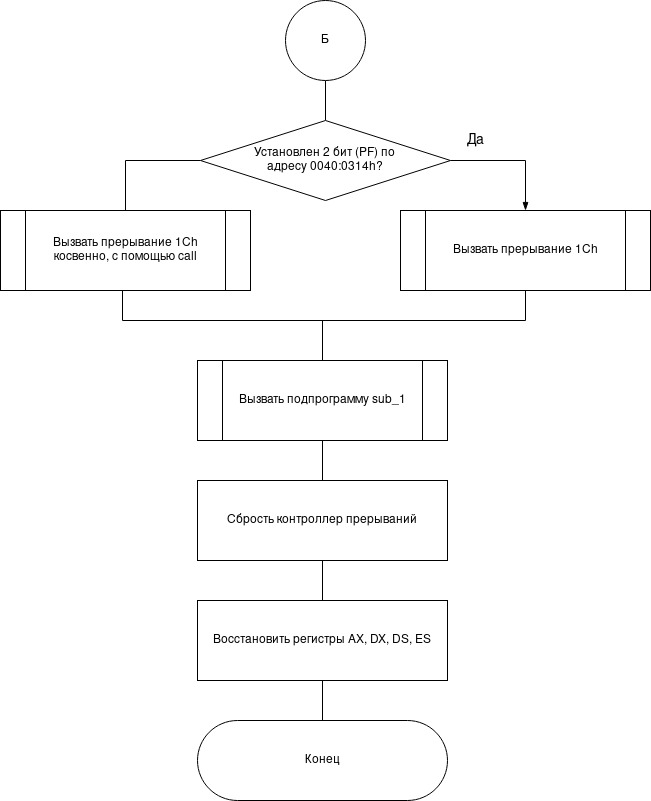
\includegraphics[scale=0.76]{../src/int8h_3.jpg}
\end{flushright}

\clearpage
\subsection{Схема алгоритма процедуры sub\_1}

\begin{center}
	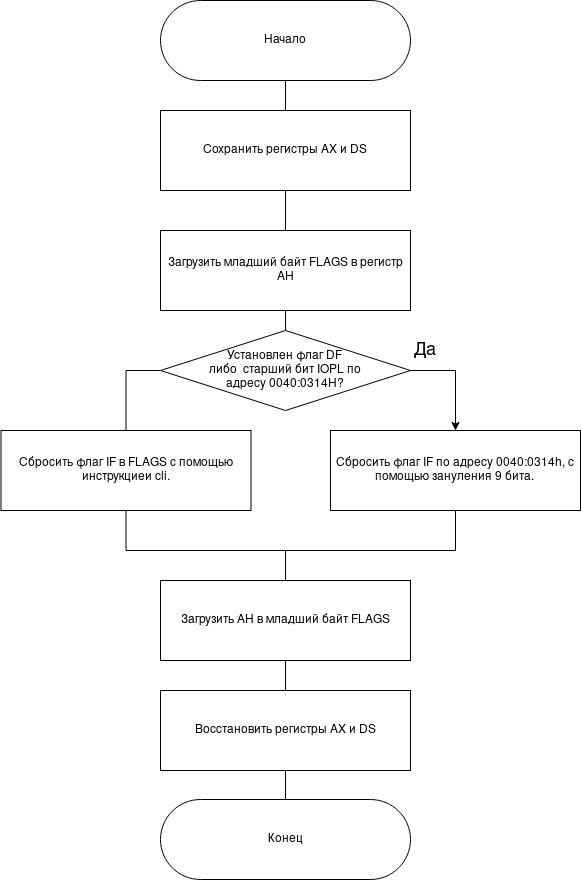
\includegraphics[scale=0.76]{../src/int8h_sub_1.jpg}
\end{center}

\end{document}